\chapter{Design of circuit}
  
  \section{DC Bias point at gate}

  We are using ADS to simulate the I-V characteristics of the CGH40010 transistor. ADS is providing a built-in design guide for this purpose. Figure~\ref{fig:fig_IV} shows the I-V characteristics, with drain current on the y-axis, drain voltage on the x-axis and curves for various gate voltages from -5 to -1 volts in 0.2 volts increments. Refering to figure 5.12 in \cite[p.~200]{AmpRobertson}, we choose to set a bias point at approximately 70\% of the maximum saturated drain current IDS, to achieve a good compromise between good linearity and high gain. We find this to be a gate voltage of about -1 volts.

  \begin{figure}[h]
	  \centering
	  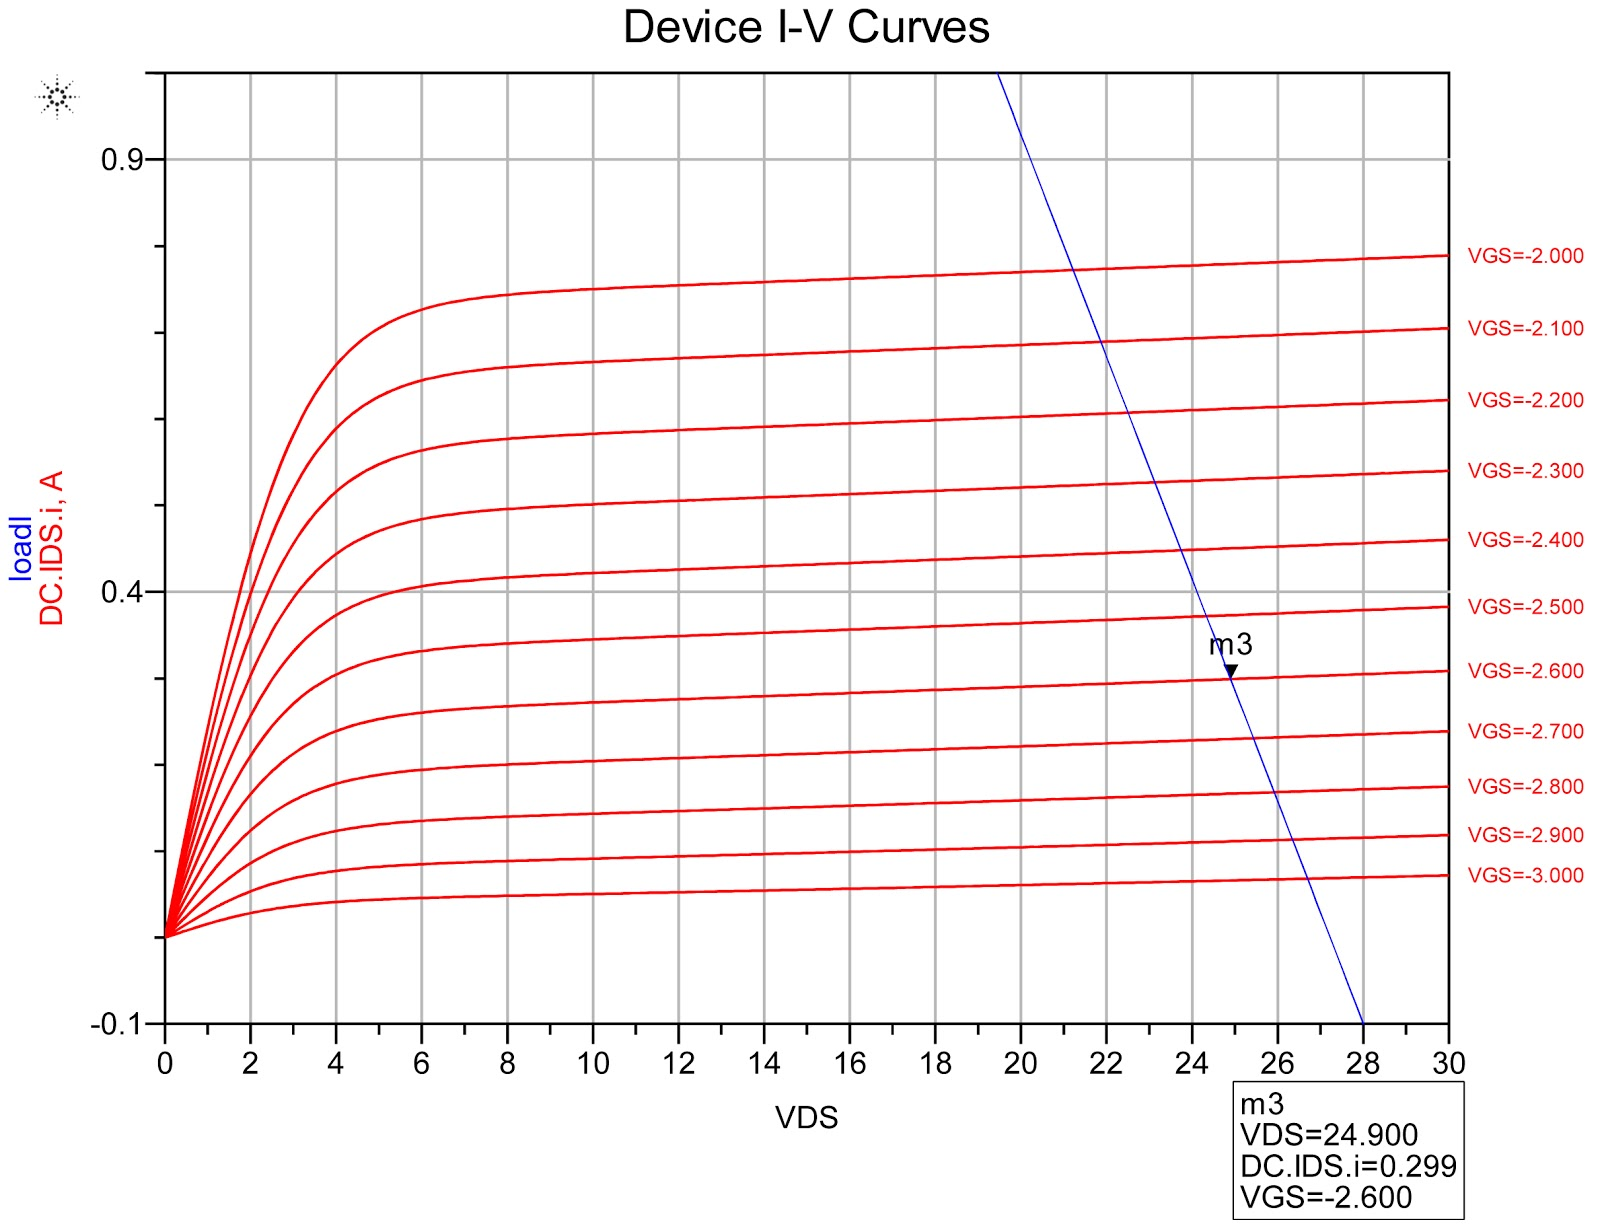
\includegraphics[width=0.75\textwidth]{img/01_IVCurve}
	  \caption{I-V curve characteristics for CGH40010}
	  \label{fig:fig_IV}
  \end{figure}

  \section{Stability}

  \subsection{Calculations}
  Table~\ref{tab:cree_sparm} lists the S-Parameters for the transistor as given in \cite{CreeDS}. Using these, we can calculate the $K$ and $\lvert \Delta \rvert$ factors to determine the stability using equations (6.31) and (6.32) in \cite{Pozar}.
  \begin{table}[h]
	  \centering
  \begin{tabular}{l l l l}
	  $S_1$$_1$ & $0.9 \angle 165^{\circ}$ & $S_{12}$ & $0.019 \angle -17.6^{\circ}$ \\
	  $S_{21}$ & $4.21 \angle 46.9^{\circ}$ & $S_{22}$ & $0.39 \angle -162^{\circ}$ \\
  \end{tabular}
	  \caption{S-parameters for Cree CGH40010}
	  \label{tab:cree_sparm}

  \end{table}

  Using these values we find $K = 0.732$ and $\lvert \Delta \rvert = 0.282$. \emph{Rollet's condition} specifies that an amplifier will be unconditionally stable if $K > 1$ and $\lvert \Delta \rvert < 1$. Since only the latter condition is fulfilled in our case, the transistor will not be unconditionally stable by itself.

  \subsection{Stabilization circuit}
  We are using a parallell RC-filter on the input to achieve unconditional stability. The circuit used is shown in figure~\ref{fig:Stabschem}. The values for R and C are found using the tune feature in ADS while observing the impact on the stability circles. A plot of the stability circles with the final values of R and C is shown in figure~\ref{fig:Stabcircle_in} and figure~\ref{fig:Stabcircle_out}. Since the stability circles are completely outside the unity circle of the Smith chart for both input and output, the amplifier is unconditionally stable in this state. The width of the microstrip lines is calculated using the Linecalc tool in ADS, to give the lines a characteristic impedance $Z_c$ of $50 \Omega$ with the substrate parameters given in this assignment.
  The stabilization circles in figure~\ref{fig:Stabcircle_out} show a possible instability for a load impedance of $Z_L \approx 0 \Omega$, ie. a short-circuit on the output. We do not consider this a major problem as a short-circuit on the output will most probably set the amplifier on fire anyways.

  \begin{figure}[H]
	  \centering
	  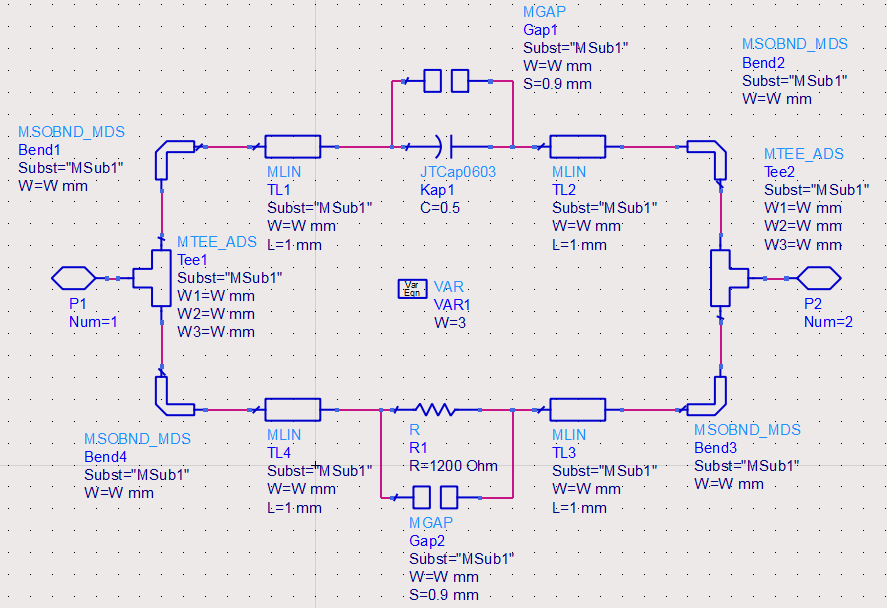
\includegraphics[width=0.8\textwidth]{img/Stabilization_circuit}
	  \caption{RC-filter for input stabilization}
	  \label{fig:Stabschem}
  \end{figure}

  \begin{figure}[H]
	  \begin{minipage}[b]{.45\textwidth}
	  \centering
	  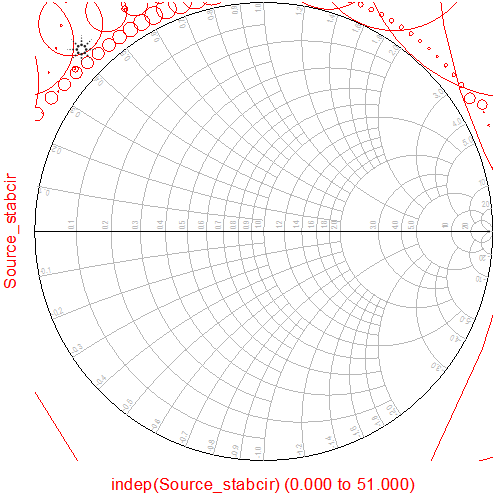
\includegraphics[width=\linewidth]{img/Stabilization_source_circle}
  	  \caption{Amplifier input stability circle}
	  \label{fig:Stabcircle_in}
  \end{minipage}%
  \begin{minipage}{.1\textwidth}
	  \hspace{\linewidth}
  \end{minipage}%
  \begin{minipage}[b]{.45\textwidth}
	  \centering
	  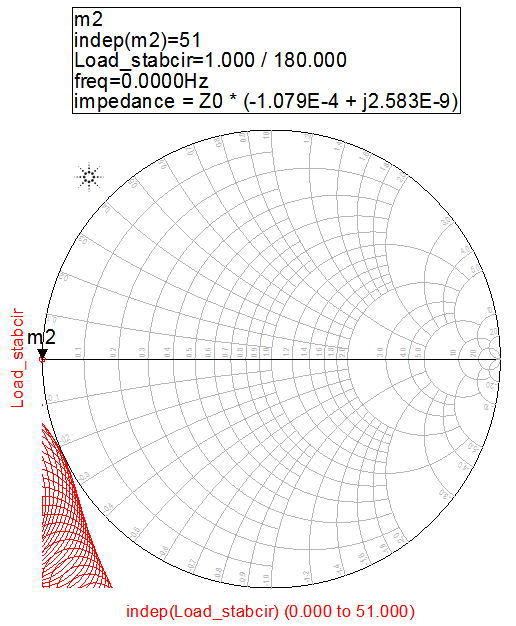
\includegraphics[width=\linewidth]{img/Stabilization_load_circle}
  	  \caption{Amplifier output stability circle}
	  \label{fig:Stabcircle_out}
  \end{minipage}
  \end{figure}

  \section{Bias network}

  The purpose of a bias network is to filter unwanted noise from the bias voltage sources to prevent it from reaching the gate and drain terminals, and to prevent RF signal from the amplifier input and output from reaching the bias voltage sources. We are using two identical bias networks for the gate and drain bias voltages, which is composed of a microstrip quarter-wave transformer which blocks the input or output signal from reaching the bias source, and a capacitor bank that filters out noise from the bias voltage sources.

  Figure~\ref{fig:Biasschem} shows the bias network we are using, with the probes used for measuring S-parameter characteristics. We have first simulated the two-port characteristics with terminal 1 at the input and terminal 2 at the point that will be connected to the transistor's gate or drain. Figure~\ref{fig:Biastwos} shows two-port parameters $S_1$$_2$ and $S_2$$_2$, which shows that within our designated frequency band from 2.35 to 2.45 GHz, only between -42 and -50 dB of the input signal gets transmitted to the bias voltage source.

  We have also simulated one-port S-parameters by grounding the input of the circuit and measuring the reflection coefficient at the output ($S_1$$_1$). This is more relevant to real-world conditions as the DC voltage source providing the bias voltage will act as an AC ground. The results of this simulation is shown in figure~\ref{fig:Biasones}. The simulation shows that within the 2.35-2.45 GHz band almost all of the incident wave is reflected, while we have a -6dB attenuation of the reflected incident wave at approx. 1.8 GHz.

  \clearpage


  \begin{figure}[h]
  	  \centering
	  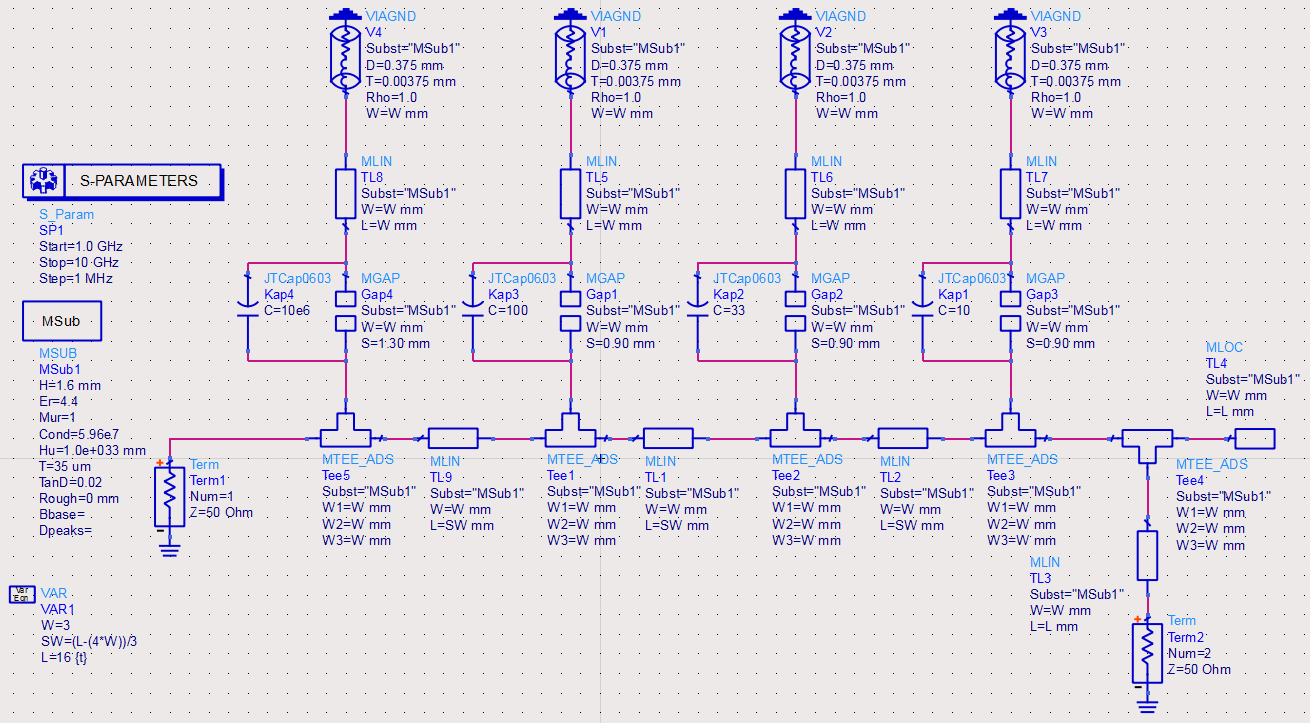
\includegraphics[width=\textwidth]{img/Bias_filter_two_port}
  	  \caption{Gate bias network schematics}
  	  \label{fig:Biasschem}
  \end{figure}

  \begin{figure}[h]
	  \begin{minipage}[b]{.45\textwidth}
	  \centering
	  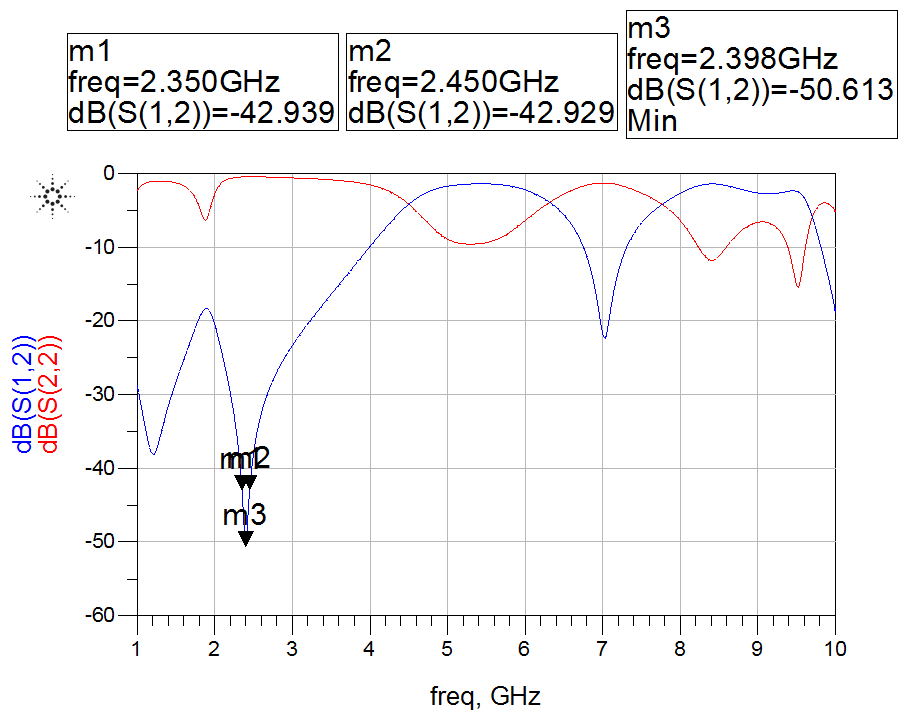
\includegraphics[width=\linewidth]{img/Bias_filter_two_port_s_parm}
	  \caption{Bias network two-port S-parameter}
  	  \label{fig:Biastwos}
  \end{minipage}%
  \begin{minipage}{.1\textwidth}
	  \hspace{\linewidth}
  \end{minipage}%
  \begin{minipage}[b]{.45\textwidth}
	  \centering
	  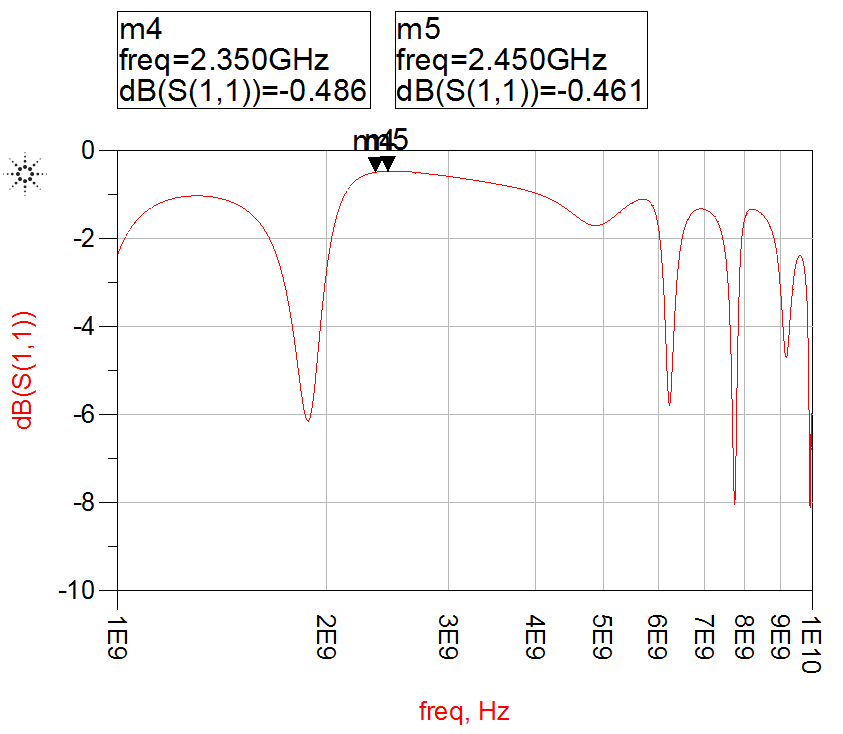
\includegraphics[width=\linewidth]{img/Bias_filter_one_port_s_parm}
  	  \caption{Bias network one-port S-parameter}
  	  \label{fig:Biasones}
  \end{minipage}
  \end{figure}


  \section{Matching network}
  Finally, to achieve the required gain specifications, the input and output of the amplifier should be impedance matched to as close as possible to $50 \Omega$. This is because the maximum power transfer occurs when both source and load have the same impedance. We are using series capacitors and shunt inductors at both input and output, which is beneficial since the series capacitors will double as DC blocking elements as well.

  \begin{figure}[h]
	  \centering
	  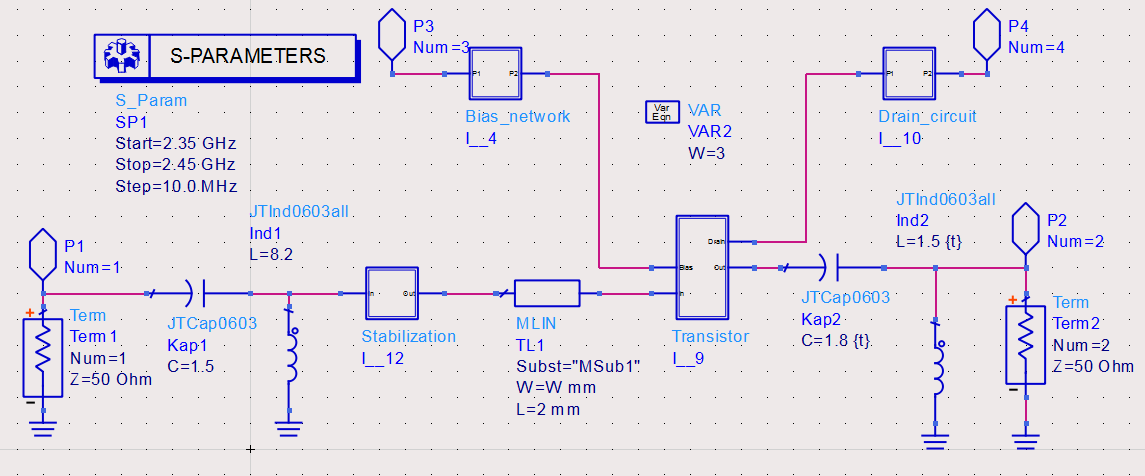
\includegraphics[width=\textwidth]{img/Matching_circuit}
	  \caption{Schematics of amplifier with matching network}
  	  \label{fig:Matchschem}
  \end{figure}

  \begin{figure}[h]
	  \begin{minipage}[b]{0.45\textwidth}
	  \centering
	  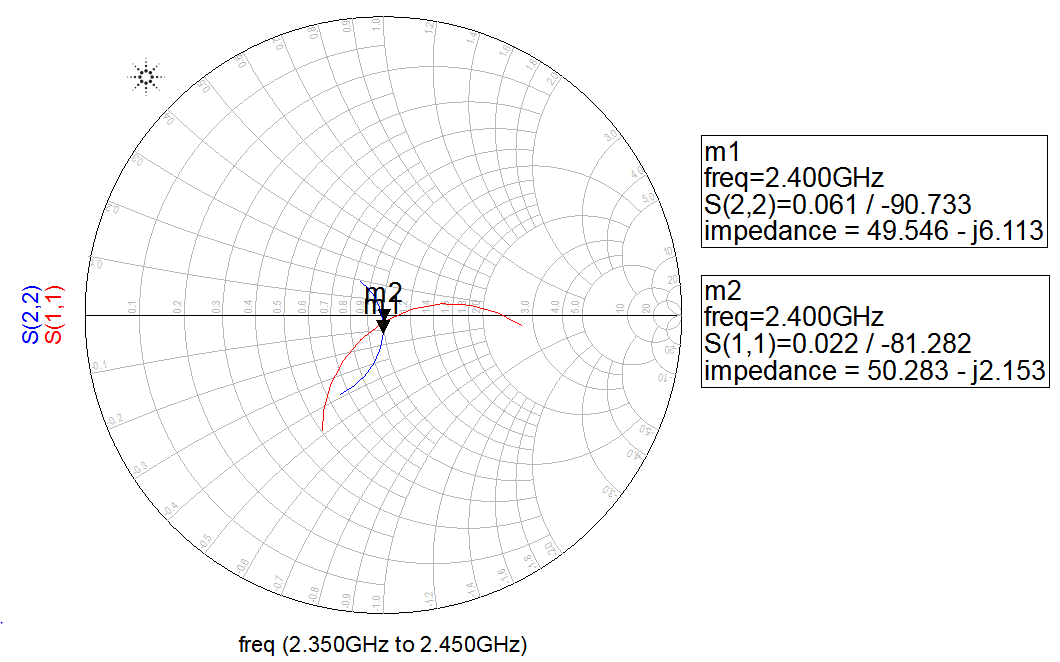
\includegraphics[width=\linewidth]{img/Matching_smith_chart}
  	  \caption{Input (red curve) and output (blue curve) impedances plotted for 2.35-2.45 GHz spectrum}
 	  \label{fig:MatchSmith}
  \end{minipage}%
  \begin{minipage}{.1\textwidth}
	  \hspace{\linewidth}
  \end{minipage}%
  \begin{minipage}[b]{0.45\textwidth}
	  \centering
	  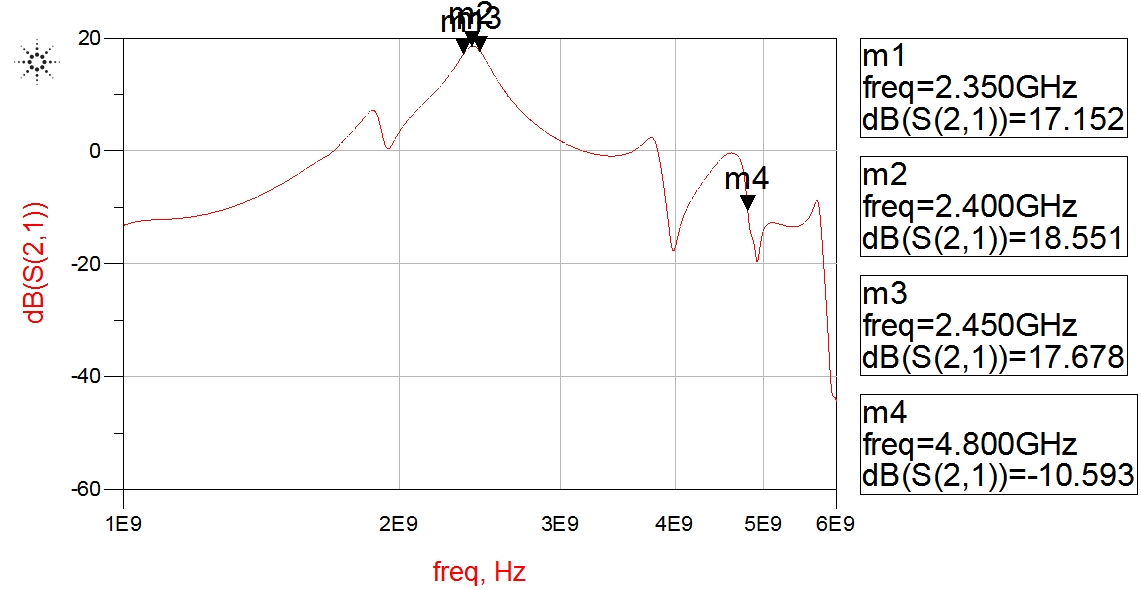
\includegraphics[width=\linewidth]{img/Small_signal_gain_matched}
  	  \caption{Gain figure for matched circuit}
  	  \label{fig:MatchGain}
  \end{minipage}
  \end{figure}
